\documentclass[11pt]{article}
\usepackage[a4paper,margin=0.8in]{geometry}
\usepackage[T1]{fontenc}
\usepackage{tikz}
\usetikzlibrary{arrows.meta,positioning,calc}
\pagestyle{empty}
\begin{document}
\begin{center}
{\LARGE\bfseries Automated Plagiarism Checker}\\[1mm]
{\large Project architecture: frontend, backend and files}
\end{center}
\begin{center}
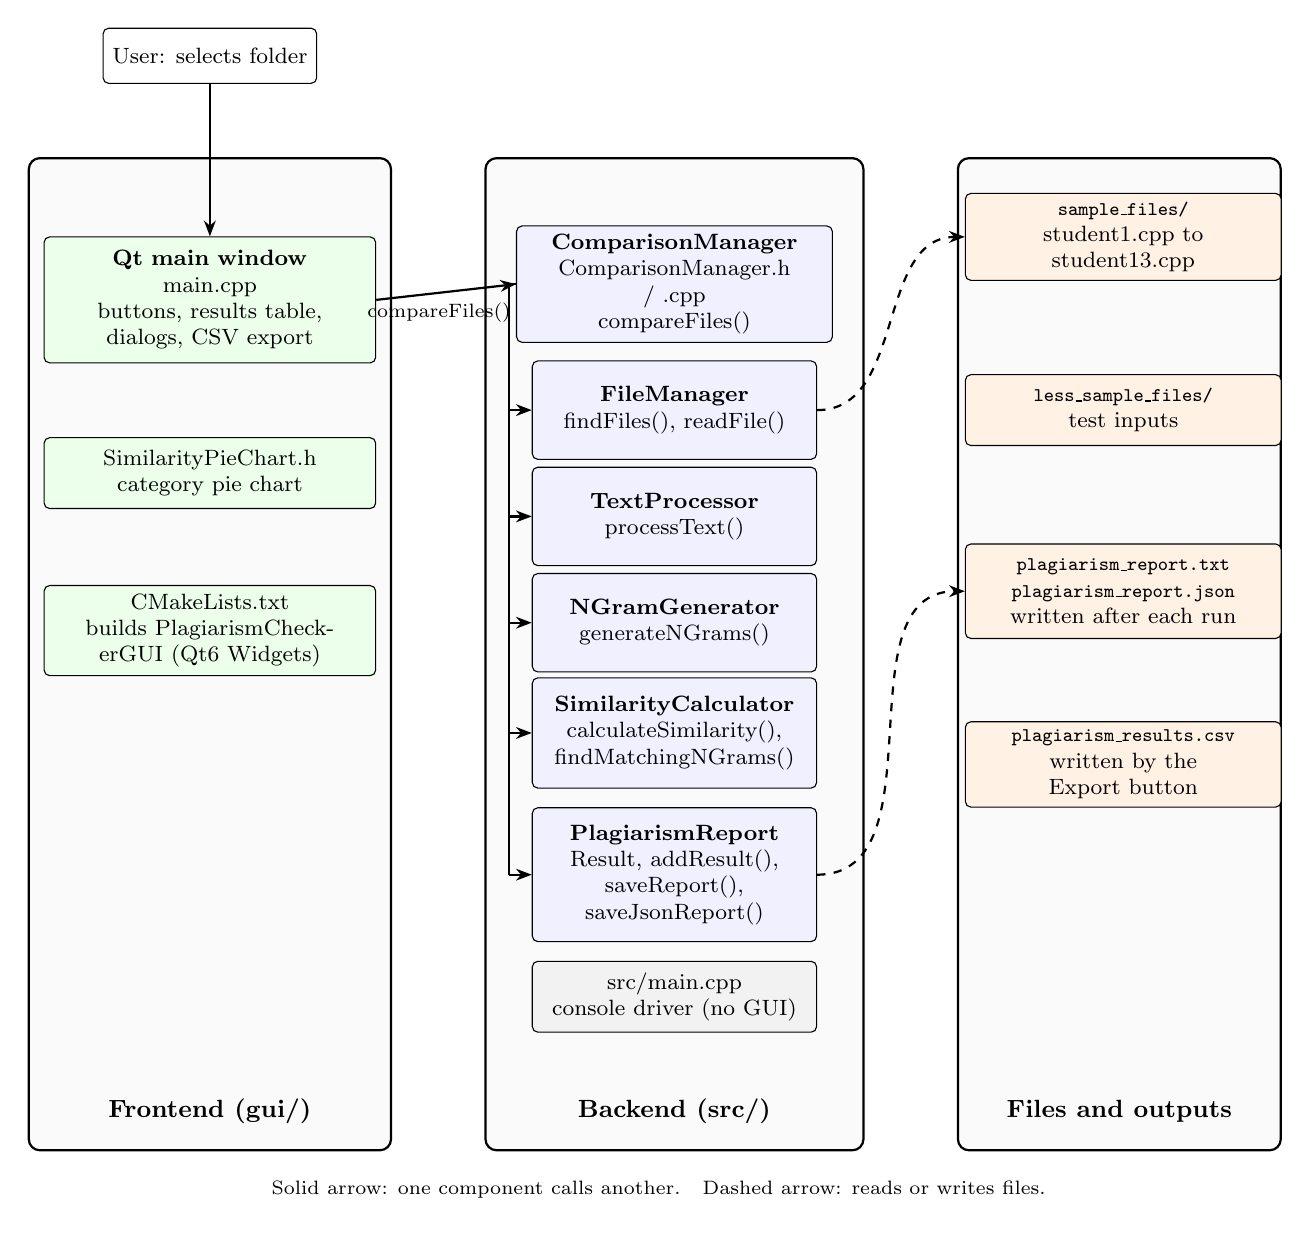
\begin{tikzpicture}[
  cont/.style={draw, rounded corners=4pt, fill=gray!4, line width=0.8pt},
  ui/.style={draw, rounded corners=2pt, fill=green!8, align=center, font=\footnotesize,
    text width=4.0cm, inner sep=3pt},
  mod/.style={draw, rounded corners=2pt, fill=blue!6, align=center, font=\footnotesize,
    text width=3.4cm, minimum height=1.25cm, inner sep=3pt},
  file/.style={draw, rounded corners=2pt, fill=orange!10, align=center, font=\footnotesize,
    text width=3.8cm, inner sep=3pt},
  call/.style={-{Stealth[length=2mm]}, thick},
  io/.style={-{Stealth[length=2mm]}, dashed, thick}
]
% ---------- containers (layers) ----------
\draw[cont] (0,-11.4) rectangle (4.6,1.2);
\draw[cont] (5.8,-11.4) rectangle (10.6,1.2);
\draw[cont] (11.8,-11.4) rectangle (15.9,1.2);
\node[font=\bfseries\small] at (2.3,-10.9) {Frontend (gui/)};
\node[font=\bfseries\small] at (8.2,-10.9) {Backend (src/)};
\node[font=\bfseries\small] at (13.85,-10.9) {Files and outputs};

% ---------- user ----------
\node[draw, rounded corners=2pt, fill=white, font=\footnotesize, minimum width=2.6cm,
  minimum height=0.7cm] (user) at (2.3,2.5) {User: selects folder};

% ---------- frontend ----------
\node[ui, minimum height=1.6cm] (gui) at (2.3,-0.6)
  {\textbf{Qt main window}\\ main.cpp\\ buttons, results table, dialogs, CSV export};
\node[ui, minimum height=0.9cm] (pie) at (2.3,-2.8)
  {SimilarityPieChart.h\\ category pie chart};
\node[ui, minimum height=0.9cm] (cmake) at (2.3,-4.8)
  {CMakeLists.txt\\ builds PlagiarismCheckerGUI (Qt6 Widgets)};
\draw[call] (user) -- (gui);

% ---------- backend ----------
\node[mod, text width=3.8cm, minimum height=1.25cm] (cm) at (8.2,-0.4)
  {\textbf{ComparisonManager}\\ ComparisonManager.h / .cpp\\ compareFiles()};
\node[mod] (fm) at (8.2,-2.0)
  {\textbf{FileManager}\\ findFiles(), readFile()};
\node[mod] (tp) at (8.2,-3.35)
  {\textbf{TextProcessor}\\ processText()};
\node[mod] (ng) at (8.2,-4.7)
  {\textbf{NGramGenerator}\\ generateNGrams()};
\node[mod, minimum height=1.4cm] (sc) at (8.2,-6.1)
  {\textbf{SimilarityCalculator}\\ calculateSimilarity(),\\ findMatchingNGrams()};
\node[mod, minimum height=1.7cm] (pr) at (8.2,-7.9)
  {\textbf{PlagiarismReport}\\ Result, addResult(),\\ saveReport(), saveJsonReport()};
\node[mod, fill=gray!10, minimum height=0.9cm] (drv) at (8.2,-9.45)
  {src/main.cpp\\ console driver (no GUI)};

% ---------- files and outputs ----------
\node[file, minimum height=1.1cm] (samples) at (13.9,0.2)
  {{\ttfamily\scriptsize sample\_files/}\\ student1.cpp to student13.cpp};
\node[file, minimum height=0.9cm] (less) at (13.9,-2.0)
  {{\ttfamily\scriptsize less\_sample\_files/}\\ test inputs};
\node[file, minimum height=1.2cm] (reports) at (13.9,-4.3)
  {{\ttfamily\scriptsize plagiarism\_report.txt}\\ {\ttfamily\scriptsize plagiarism\_report.json}\\ written after each run};
\node[file, minimum height=1.0cm] (csv) at (13.9,-6.5)
  {{\ttfamily\scriptsize plagiarism\_results.csv}\\ written by the Export button};

% ---------- calls: frontend to backend ----------
\draw[call] (gui.east) -- node[below, font=\scriptsize, pos=0.45] {compareFiles()} (cm.west);
\draw[thick] (cm.west) -- (6.1,-0.4) -- (6.1,-7.9);
\draw[call] (6.1,-2.0) -- (fm.west);
\draw[call] (6.1,-3.35) -- (tp.west);
\draw[call] (6.1,-4.7) -- (ng.west);
\draw[call] (6.1,-6.1) -- (sc.west);
\draw[call] (6.1,-7.9) -- (pr.west);

% ---------- file access ----------
\draw[io] (fm.east) to[out=0, in=180] (samples.west);
\draw[io] (pr.east) to[out=0, in=180] (reports.west);

% ---------- legend ----------
\node[font=\scriptsize, align=center] at (8.0,-11.9)
  {Solid arrow: one component calls another.\quad Dashed arrow: reads or writes files.};
\end{tikzpicture}
\end{center}
\end{document}
